%\documentclass[11pt]{article}
\documentclass{asme2ej}
\usepackage{amsmath,amssymb,graphicx,bm}
\usepackage{listings, color, subcaption, placeins}
\usepackage{undertilde}
\usepackage{algorithm,algpseudocode}
\usepackage{multicol}
\usepackage{makecell}
\usepackage{pgfgantt}
\usepackage[table]{colortbl}
\graphicspath{{./images}}
%%%%%%%%%%%%%%%%%%%%%%%%%%%%%%
%%%%%%%%%%%%%%%%%%%%%%%%%%%%%%
%%%%%%%%%%%%%%%%%%%%%%%%%%%%%%

%% If you want to define a new command, you can do it like this:
\newcommand{\Q}{\mathbb{Q}}
\newcommand{\R}{\mathbb{R}}
\newcommand{\Z}{\mathbb{Z}}
\newcommand{\C}{\mathbb{C}}
\newcommand{\e}{\bm{e}}
\newcommand{\TEN}[1]{\underline{\underline{#1}}}
\newcommand{\VEC}[1]{\utilde{#1}}
\newcommand{\UVEC}[1]{\underline{#1}}
\newcommand{\PK}[1]{\TEN{\tau}^{(#1)}}
\newcommand{\cauchy}{\TEN{\sigma}}
\newcommand{\st}{$^{\text{st}}$}
\newcommand{\nd}{$^{\text{nd}}$}
\newcommand\defeq{\mathrel{\stackrel{\makebox[0pt]{\mbox{\normalfont\tiny def}}}{=}}}

\graphicspath{{./images/}}

%% If you want to use a function like ''sin'' or ''cos'', you can do it like this
%% (we probably won't have much use for this)
% \DeclareMathOperator{\sin}{sin}   %% just an example (it's already defined)


\begin{document}
\title{Users Manual}
\author{Nathan Miller}

\maketitle

Included with the user element is a simple driver program which can be used to test the element's capabilities. This driver program uses input files (*.inp) which have several keywords available for use.

\section{Comments}

Comments are indicated by a \verb|#| symbol at the beginning of the line. If this is encountered first all information in the line is ignored. Note that in line comments after input commands are not currently supported.

\section{*NODES}

*NODES allows the user to define a node of the finite element model. Only 3D nodes are currently supported. An example input is

\begin{verbatim}
*NODES,12
1, 1.2, 2.3, 5.4
3, 6.5, 7.6, 2.1
\end{verbatim}

This creates two nodes with 12 degrees of freedom at each node (the 12 next to *NODES). These nodes have $x$, $y$, $z$ coordinates given after the node number. Note that the node numbers do not have to necessarily be in order.

\section{*DIRICHLET\_BCS}

*DIRICHLET\_BCS allows the user to define Dirichlet type boundary conditions on the mesh. This forces a degree of freedom to assume the value given in the code. These can either be defined using a nodeset or a single node

\begin{verbatim}
*DIRICHLET_BCS
nodeset, bottom, 3, 0.0
1, 2, 3.
\end{verbatim}

In this example two different approaches are used. The first indicates that for all nodes in the nodeset, ``bottom,'' the third degree of freedom is held at zero.

The second approach indicates that the second degree of freedom at node 1 should be set to 3.

\section{*ELEMENTS}

*ELEMENTS allows the user to define elements in the model. Elements should be defined with the nodes incrementing in a, ``clockwise,'' manner (see Figure~\ref{fig:node_numbering}).

\begin{verbatim}
*ELEMENTS
1,2,4,6,3,7,10,11,9
\end{verbatim}

The first value is the element number, and the remainder are the node numbers.

\begin{figure}
\centering
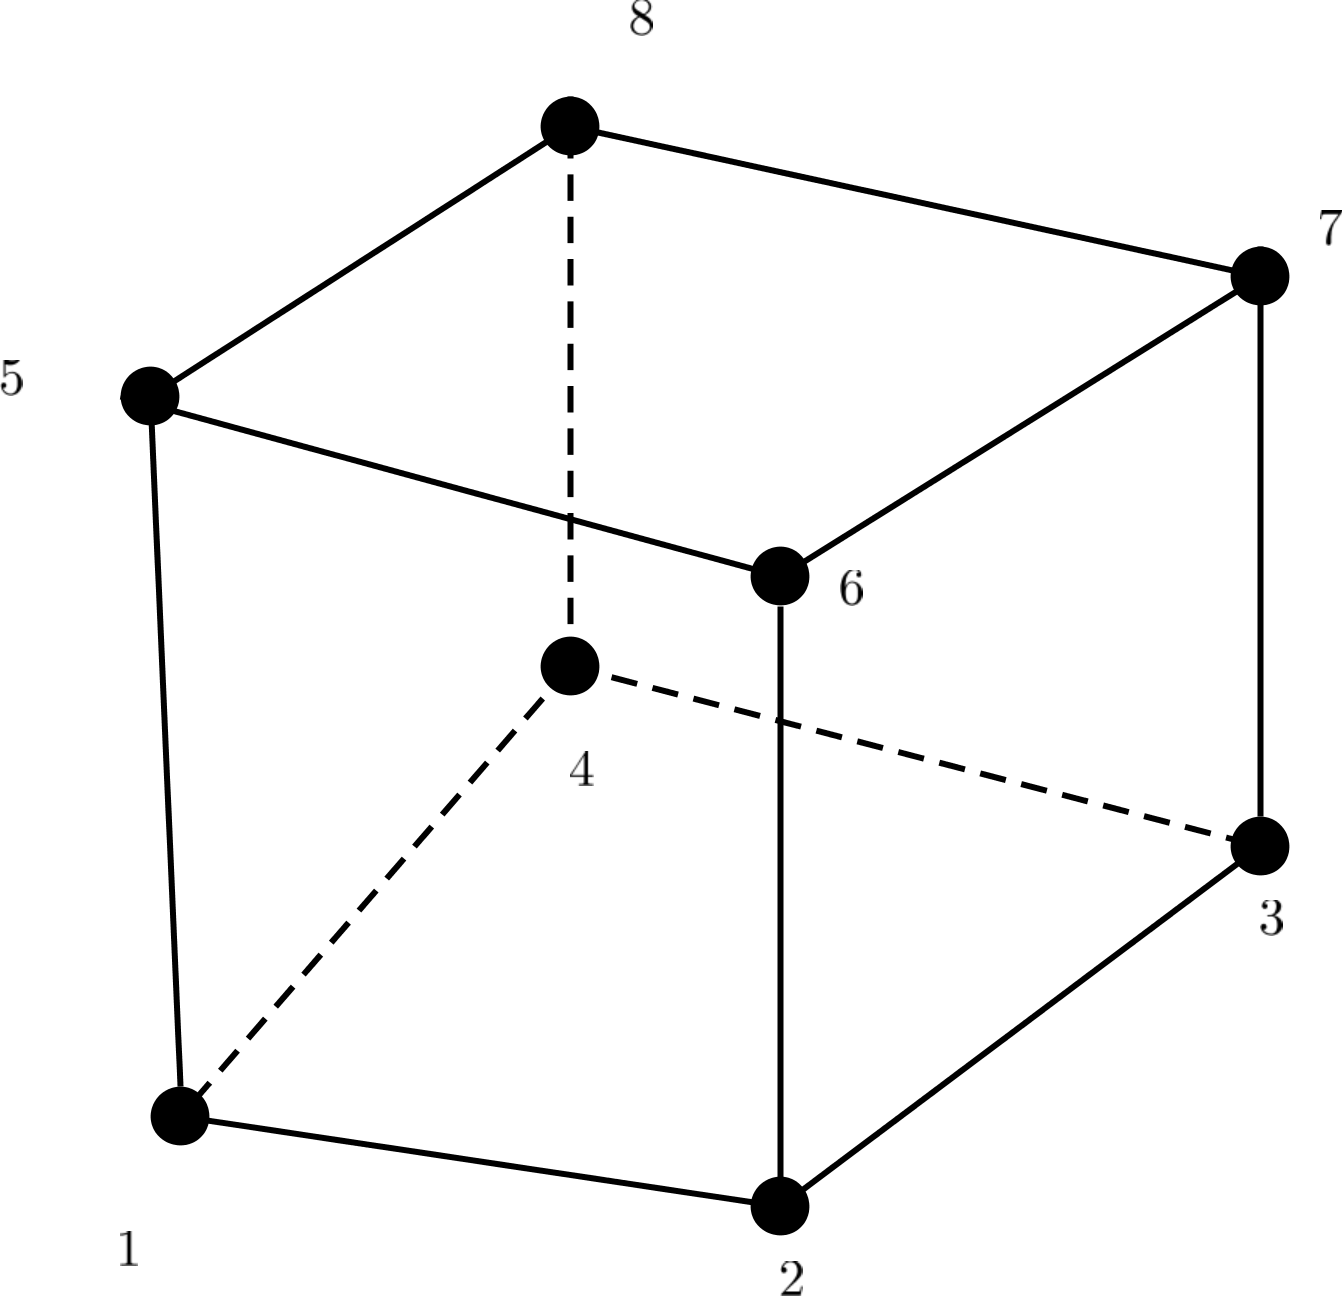
\includegraphics[width=0.5\textwidth]{./element.png}
\caption{Element node numbering}
\label{fig:node_numbering}
\end{figure}

\section{*PROPERTIES}

*PROPERTIES allows the user to define the material properties used in the constitutive model. There can be any number of properties but they currently can only be on one line. Properties can also only be defined once.

\begin{verbatim}
*PROPERTIES
1,4,1,5,2,6,1,.2,5,1.2,...
\end{verbatim}

The current material model (linear elasticity) takes 19 parameters. They are the initial density, $\lambda$, $\mu$, $\eta$, $\tau$, $\kappa$, $\nu$, $\sigma$, $\tau_1$, $\tau_2$,  $\tau_3$, $\tau_4$, $\tau_5$, $\tau_6$, $\tau_7$, $\tau_8$, $\tau_9$, $\tau_{10}$, and $\tau_{11}$.

\section{*LATEX}

*LATEX allows the user to input LaTeX typesetting code for use in documentation of the simulation. This is important to use for any additional regression tests which may be developed so that future users have a clear understanding of what is being tested. An example command is given below

\begin{verbatim}
*Latex
The user can put LaTeX commands in the following lines. The code
allows the user to input general latex commands which will then 
be copied into a file.

Empty lines spaces are okay though they will not be recognized 
as such.
\end{verbatim}

\section{*NSET}

This allows the user to define nodesets or collections of nodes which have similar boundary conditions or other properties assigned to them.

\begin{verbatim}
*NSET
bottom,      1,  2,  3,  4
top,         5,  6,  7,  8
front,       1,  2,  5,  6
\end{verbatim}

There can be any number of nodesets defined after the *NSET command

\section{*MMS}

Allows the user to indicate that the simulation is to use the method of manufactured solutions for code verification.

\begin{verbatim}
*MMS,const_u
mms_set,1,2,3,4,5,6,7,8,9,10,11,12,13,15,16,17,18,19,20,21,22,23,24,25,26,27
\end{verbatim}

The first line should contain the name of the function (only const\_u and linear\_u are currently recognized) to be used. The second line defines a nodeset which encompasses all of the nodes on the boundary of the model.

\FloatBarrier

\bibliographystyle{asme2ej}
\bibliography{mpm}

\end{document}